\documentclass[a4paper,twocolumn,10pt]{article}
\usepackage[margin=1in]{geometry}
\usepackage{listings}
\usepackage[utf8]{inputenc} % allow utf-8 input
\usepackage[T1]{fontenc}    % use 8-bit T1 fonts
\usepackage{hyperref}       % hyperlinks
\usepackage{url}            % simple URL typesetting
\usepackage{booktabs}       % professional-quality tables
\usepackage{amsfonts}       % blackboard math symbols
\usepackage{nicefrac}       % compact symbols for 1/2, etc.
\usepackage{microtype}      % microtypography
\usepackage{lipsum}     % Can be removed after putting your text content
\usepackage{graphicx}
\usepackage{titlesec}
\usepackage{fancyhdr}
\usepackage{siunitx}
\usepackage{amsmath}

\pagestyle{fancy}
\titleformat{\section}{\large\scshape}{\thesection}{1em}{}
\titleformat{\subsection}
  {\normalfont\scshape}{\thesubsection}{1em}{}
\titleformat{\subsubsection}
  {\normalfont\scshape}{\thesubsubsection}{1em}{}
\pagenumbering{arabic}
\newtheorem{definition}{Definition}[section]
\usepackage[backend=biber,style=ieee,natbib=true]{biblatex}
\renewcommand{\bibfont}{\footnotesize} % for IEEE bibfont size
\addbibresource{citations.bib} %added

\usepackage{csquotes}

\title{\vspace{-50pt}\bfseries{\Large{Midi Shark: For Piano Transcription}}}
\author{\normalfont{Jonah Chen, QiLin Xue, Joe Hattori, Khanatat Thangwatthanarat}\\\small{University of Toronto}\\\vspace{-10pt}\small{\url{{jonah.chen,qilin.xue,joe.hattori,k.thangwatthanarat}@mail.utoronto.ca}}}
\date{\today}
\begin{document}
\maketitle
\section{Introduction}
Transcription of music is the process of determining the pitches and timing of notes from recorded audio files. Transcription has always been a specialized task that requires years of musical training. Transcription is even more challenging for polyphonic music, such as piano, which features the simultaneous production of two or more tones. The majority of traditional transcription models focus on extracting all of the notes from the recording using the node onset. This, however, is not the way a trained musician approaches the problem\cite{intro}.

We developed a model that is more accurate at transcribing piano recordings by analyzing the recording with a neural network and focusing on both the onsets and offsets of the node. Moreover, since images and audios both have common two-dimensional time-frequency input representations, the fact that CNN performs well in image classification problems suggests that CNN could potentially be used for music transcription\cite{onsets_and_frames}.

\section{Illustration}
The model architecture is shown in figure \ref{fig:architecture}.
\begin{figure}[h!]
  \centering
  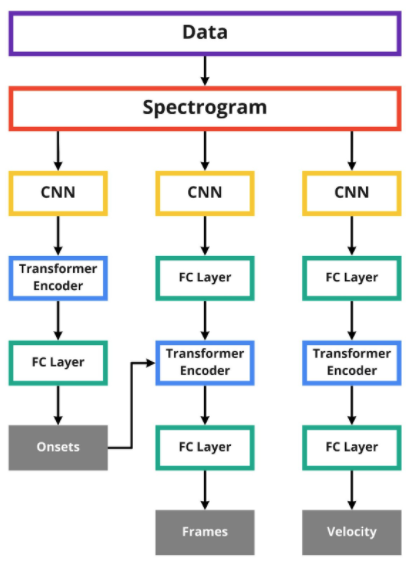
\includegraphics[width=0.7\linewidth]{figures/architecture.png}
  \caption{Model architecture}
  \label{fig:architecture}
\end{figure}

\section{Background}
Polyphonic automatic music transcription is a difficult task due to the potential of having multiple notes played simultaneously, causing the harmonics of each note to overlap with the others. Therefore, it is a non-trivial task to transcribe the music using the spectrogram. 

Since the advent of machine learning, there have been models developed for solving this problem. A relatively successful model is the Onsets and Frames (OF) model developed by the Google Brain Team using TensorFlow in 2017 and implemented into the open-source “magenta” framework[9]. This model uses a two-headed encoder-decoder architecture that predicts onsets (when the notes are played), and frames (what notes are played at the onset). This model uses convolutional neural networks as encoders and bidirectional LSTM as decoders and was able to achieve an F1 score of 78.30\% and 82.29\% on frames and notes respectively for the MASTERO dataset, which is arguably the largest dataset for music transcription task.

\section{Data Processing}
We used Maestro Dataset as the Google Brain Team did to develop the OF model. This dataset consists of pairs of WAV files and MIDI files of piano audio, and in total, they amount to 200 hours.
WAV files are raw audio files, and corresponding MIDI file contains labeled information of each WAV file, such as when, what and how strong each note was played.

We treated MIDI files as the ground truth; our model takes WAV files as the input, and trains against the MIDI files. However, both file types are hard for the model to understand, so we needed to perform data processing to begin with.

Our data processing can be broken down to two major parts. One is converting WAV files to spectrograms, and the other task is converting MIDI files to a certain kind of form which is easier to train the model.

We chose to convert MIDI files into arrays with time on the x-axis and note on the y-axis. As MIDI files hold when each note begins, how long it lasts, and how strong it was played, we divided MIDI files into three arrays respectively; first array is onsets array, the second array is frames array, and the third array is velocity array.

Since every song has a different length, we divided all the spectrograms and the labels into 20 second segments, so our model will take a 20 second long spectrogram as input.

The downside of this approach is that we might have a clip at the end of the song that is shorter than 20 seconds. This can be resolved by zero-padding, however, since most songs were several minutes long, we did not think this would make a noticeable difference and opted to simply ignore these last few seconds.
\section{Architecture}
The OF model\cite{onsets_and_frames} had seen success in the task of automatic music transcription, but since 2017 when the model was published, there have been several publications that have brought forth improvements in areas like sequence processing.

In the OF model, the processed mel-spectrogram data is encoded using a stack of convolutional layers\cite{rainer}. Furthermore, the OF model uses bidirectional LSTM models as decoders. Since 2017, the transformer architecture has revolutionized the processing of sequential data\cite{attention}. Many of today’s state-of-the-art models in fields like natural language processing are based on the transformer. As audio is sequential data, we think it will be advantageous to use a transformer encoder in place of the bidirectional LSTM.

Following similar data flow to OF, we will have a two-headed model with an onset and frame head. The onset prediction is passed as an input to the transformer encoder that decodes the frame predictions. We use the same loss functions for the two heads from OF (a generalization of cross-entropy loss, see eq.1-6 in\cite{onsets_and_frames}). For the velocity model, we use a similar approach to the frames model but without the input from onset prediction. Apart from that, we use the modified version of mean square error instead of a cross-entropy loss as a loss function. For all the models, we use Adam optimizer as our optimization function.  For all the models, we also use fully connected layers in between. For a clearer picture of the model structure, please refer to figure 1 in the introduction section.

\section{Baseline Model}



\section{Quantitative Results}



\begin{center}
    \begin{tabular}{|c|c|}
        \hline
        Model& Frames F1 Score \\
        \hline
        Sigtia et al., 2016 & \(72.22\%\)\\
        \hline
        Kelz et al., 2016 & \(71.60\%\)\\
        \hline
        Melodyne\footnote{Commercial software, not machine learning model.} & \(58.57\%\)\\
        \hline
        Google’s 2017 Model & \(78.30\%\)\\
        \hline
        \textbf{Google’s 2021 Model} & \(\mathbf{82.18\%}\)\\
        \hline
        Midi Shark (Us) & \(79.01\%\)\\
        \hline
    \end{tabular}
\end{center}

\section{Testing}


\section{Discussion}
\section{Ethical Considerations}
In the United States, the music sheet industry is worth around 1 billion USD\cite{musicspoke}. A technology that can transcribe music may render purchasing music sheets useless. Many of these sales come from music books, which often contain several scores that can be readily found online, so big publishers will likely not be greatly affected by this technology.

However, this technology will negatively affect small composers, who may make a living by selling sheet music to their music, for example on services such as MusicSpoke\cite{musicspoke}. If this technology is accurate and readily available, it may encourage musicians to automatically generate the sheet music to the songs they like, instead of purchasing and supporting artists. Fortunately, transcribing isn’t just about having the right notes, but the style in which it is presented. This is why two transcribers will not produce the same sheet music for the same song.

The MASTERO dataset and the scope of our project consist of working solely with music, so there is a low risk of discriminating against humans from pre-processing to training and post-processing. However, a large majority of the music from the dataset is Western music, so the results would likely be more reliable towards Western music. Thus, people from other cultures may not find the same success in this model as people in Western cultures do. To address this, we will attempt to find other similar datasets that were trained on music from other cultures.

\section{References}


\printbibliography
\end{document}